% Locality Gates Dimensionality -- arXiv manuscript (port of PAPER.md v0.2)
% Build: tectonic main.tex
\documentclass[11pt]{article}

\usepackage[margin=1.1in]{geometry}
\usepackage{mathptmx}
\usepackage[T1]{fontenc}
\usepackage{amsmath,amssymb}
\usepackage{graphicx}
\usepackage{booktabs}
\usepackage{xcolor}
\usepackage[round]{natbib}
\usepackage{tikz}
\usetikzlibrary{shapes.geometric,arrows.meta,positioning}
\usepackage[colorlinks=true,linkcolor=blue!60!black,citecolor=blue!60!black,urlcolor=blue!60!black]{hyperref}

\newcommand{\Wstar}{W^{*}}
\newcommand{\pholm}{p_{\mathrm{Holm}}}

\title{Locality Gates Dimensionality:\\ When (and Why) a 2D Computational Medium\\ Beats Its 1D Serialization}
\author{Yoshihiro Sakatani\\ \small sdtech Inc. \\ \small \texttt{sakatani.yoshihiro@sdtech.co.jp}}
\date{July 2026}

\begin{document}
\maketitle

\begin{abstract}
Does laying a problem out in two dimensions help a neural network reason about
it? Prior work returns conflicting answers because it conflates three separate
questions: whether 2D structure helps as an \emph{input encoding}, as a
\emph{computational medium}, and as a \emph{learned representation}. We
disentangle them with a sequence of pre-registered experiments in which every
model arm consumes the same lossless information and arms differ only in the
connectivity of their operator. We find that \emph{locality gates
dimensionality}: a 2D layout confers a computational advantage if and only if
the operator is constrained to be spatially local, and the task's dependency
structure has low bandwidth in 2D but high bandwidth under every 1D
linearization. Under these conditions the advantage is large and robust: a
2D-local operator solves iterative relational tasks at twice the problem width
of a parameter- and window-matched 1D-local operator (a gap that survives a
space-filling-curve control), and a 2D-local rule trained on small grids
transfers to unseen grids up to $11\times$ larger in area across three task
families (connectivity, metric, dynamics) while its 1D counterpart drops to
chance; all headline effects hold at 5 seeds under Holm correction
($p < 2\times10^{-5}$). A depth taxonomy sharpens the picture: transfer is
\emph{flat} when the task's intrinsic computation depth is bounded, and
\emph{fades} only when required depth scales with problem size. Outside these
conditions the advantage vanishes: global attention erases it in-distribution
(while a curriculum-trained iterative Transformer that masters the training
sizes still transfers nothing to larger ones), recurrent message passing on
given graphs already size-generalizes without any layout (a boundary we
reproduce in-house: a stabilized recurrent GNN reaches 1.00 at every width on
given-graph reachability), and learned differentiable placements of implicit
structure lose to a set-transformer. We compile these results into a decision procedure for when a
2D-local computational medium is the right inductive bias, and argue that its
practical home is native-grid, locality-constrained computation rather than
general relational reasoning.
\end{abstract}

\section{Introduction}\label{sec:intro}

Two-dimensional layouts are ubiquitous in human reasoning artifacts ---
blueprints, circuit diagrams, board games, spreadsheets --- and a classical
argument holds that diagrams support reasoning \emph{computationally}, by
making related items adjacent so that inference requires only local search
\citep{larkin1987diagram}. Modern deep learning offers a natural test bed for
this hypothesis: does giving a neural model a 2D arrangement of a relational
problem, rather than a 1D serialization of the same content, improve its
reasoning?

The question is not academic: the field currently bets on both sides of it
daily. Vision Transformers serialize images into 1D patch sequences, discard
the convolutional locality prior, and win at scale, explicitly framing
large-scale training as trumping inductive bias \citep{dosovitskiy2021vit};
neural PDE surrogates and cellular automata bet on local 2D operators; and
the default practice of the LLM era is to serialize grid-structured worlds
--- tables, boards, ARC-style puzzles --- into token streams, where their
difficulty is a live concern. Our own program produced both answers in
consecutive pre-registered phases: a null for 2D structure under global
attention, and a large positive under a locality constraint, reconciled only
once the question was conditioned properly.

Empirically, then, the question is unsettled, and we argue this is because it
is usually posed without controlling \emph{what kind} of 2D usage is at
stake:

\begin{enumerate}
\item \textbf{2D as input encoding.} Tokens carry $(x, y)$ features; the
  operator is global attention. Here a set of positioned tokens is
  computationally just ``a set with two extra features,'' and
  permutation-invariant attention is already robust to the geometric
  transformations (e.g.\ translation) that 2D structure is supposed to buy. In
  our own earlier pilot (summarized in \S\ref{sec:boundary-global}),
  three operationalizations of a 2D positional bias all failed to beat a plain
  set-attention baseline.
\item \textbf{2D as computational medium.} The state lives on a 2D field and
  the operator is \emph{spatially local} (convolution, windowed attention,
  cellular automaton). Now the layout determines which interactions are cheap:
  locality makes dimensionality matter.
\item \textbf{2D as learned representation.} The model must \emph{discover} a
  2D placement of structure that is not natively spatial. This adds a hard
  joint optimization on top of (2).
\end{enumerate}

These three regimes are not an ad-hoc list: they are cells of a $2 \times 2$
design spanned by two orthogonal axes, \emph{operator connectivity}
(global vs.\ local) and \emph{layout provenance} (given vs.\ learned). The
fourth cell --- a learned layout consumed by a global operator, familiar as
learned positional embeddings in Transformers --- is degenerate under this
paper's headline result: without locality, position is a feature rather than
a schedule, and the cell inherits the verdict of regime (1). A scope note:
throughout, we ask whether a 2D layout helps the model \emph{compute}; uses
of 2D as an output or interface representation for humans (diagrams,
visualizations) are a separate question and out of scope.

This paper's contribution is a controlled, pre-registered characterization of
regime (2), together with boundary experiments delimiting it against (1) and
(3). Our headline finding is conditional: the 2D advantage exists, is large,
and is mechanistically explainable, but only inside a regime whose boundaries
we can state precisely. We map that regime; we do not advocate beyond it.

Concretely, we contribute:

\begin{itemize}
\item \textbf{Mechanism I --- bandwidth separation
  (\S\ref{sec:mech1}).} On a $W \times W$ grid, the dependency graph of a
  local iterative computation has bandwidth 1 under the 2D layout but
  bandwidth $\ge \min(W, H)$ under \emph{every} 1D linearization
  \citep{chvatalova1975optimal}. At matched parameters, window size, and
  depth, a 2D-local operator clears a reachability task at threshold-width
  $\Wstar = 8$ versus $\Wstar = 4$ for its 1D-local counterpart --- and a
  space-filling-curve (Hilbert-style) serialization does not close the gap
  ($\Wstar = 4$), turning the graph-bandwidth theorem into an observed floor.
\item \textbf{Mechanism II --- scale-equivariance and length-generalization
  (\S\ref{sec:mech2}).} A weight-shared 2D-local rule is the \emph{same
  computation} at every grid size, whereas a 1D serialization couples the
  learned kernel to the width $W$ (a vertical neighbor sits $W$ positions
  away). Trained on $W \le 6$ and tested up to $W = 20$, 2D-local operators
  retain 0.73--0.96 accuracy across three task families while the matched 1D
  operator is at chance on every unseen size.
\item \textbf{Mechanism III --- a depth taxonomy (\S\ref{sec:mech3}).} Whether
  transfer is flat or fading is predicted by whether the task's intrinsic
  computation depth is bounded (local dynamics, fixed-radius metric queries:
  flat at 0.89--0.96) or scales with problem size (reachability: fades under a
  fixed budget). An adaptive-depth neural cellular automaton does not rescue
  the scaling case; the depth bound is a property of the task class rather
  than a fixable artifact.
\item \textbf{Boundary map (\S\ref{sec:boundary}).} Three pre-registered
  negative results delimit the regime: (i) removing the locality constraint
  (global attention) erases the advantage; (ii) when the sparse graph is
  \emph{given}, recurrent message passing already size-generalizes up to
  $1000\times$ without any spatial layout \citep{groetschla2022recurrent} ---
  no room for a 2D win; (iii) when the layout must be \emph{learned} from
  implicit structure, a differentiable Sinkhorn placement trains but
  underfits, and a set-transformer beats it.
\item \textbf{A decision procedure (\S\ref{sec:decision})} that a
  practitioner can apply to predict whether a 2D-local medium will help on
  their task.
\end{itemize}

A methodological note: every gate in this program was pre-registered (win/null
thresholds committed to version control before the corresponding run), with
matched-information and matched-budget constraints (\S\ref{sec:protocol}), and
with purpose-built controls: a space-filling-curve serialization, a
1D-intrinsic task, a GNN positive control, and a random-layout control.
Several of the controls changed the conclusions
(\S\ref{sec:serialization}, \S\ref{sec:control-caught},
\S\ref{sec:boundary-layout}); we report the null and inconclusive outcomes
alongside the positives.

\paragraph{What this paper does not claim.} Our results do not support the
reading that ``2D representations reason better than Transformers'': under
global attention the layout is irrelevant (\S\ref{sec:boundary-global}), and
nothing here bears on large-scale language models. Nor do we claim that
2D-local operators beat graph networks in general: on given graphs,
stabilized recurrent GNNs size-generalize without any layout
(\S\ref{sec:boundary-given}), and our own GNN arm is a plain fixed-depth
message-passing network used as a learnability control rather than a
representative of the strongest graph methods (\S\ref{sec:mech2},
\S\ref{sec:robustness});
when edges must instead be \emph{estimated} from features, the estimated
graph itself degrades with size (\S\ref{sec:boundary-layout}). The claims are
exactly the conditional ones: among matched local operators, on tasks with
the stated bandwidth structure, the 2D layout wins, transfers across scale,
and does so for stateable reasons.

\section{Related work}\label{sec:related}

\paragraph{Size- and length-generalization.} GNNs trained on small graphs
often fail on larger ones \citep{yehudai2021local}; the number of
message-passing rounds bounds what graph problems are solvable at all
\citep{loukas2020depth}. Recurrent architectures with stabilization
extrapolate dramatically better: \citet{schwarzschild2021canyou} on mazes and
prefix sums with recurrent CNNs, IterGNN \citep{tang2020itergnn}, and most
relevantly \citet{groetschla2022recurrent}, whose recurrent GNNs
(skip-to-input, $L_2$ state regularization, edge convolutions) extrapolate to
graphs $1000\times$ larger on path, prefix-sum, and distance tasks. Our
\S\ref{sec:boundary-given} treats this as a boundary condition: on
\emph{given} sparse graphs the size-generalization problem is substantially
solved without any spatial layout. Benchmarks such as CLRS-30
\citep{velickovic2022clrs} formalize the out-of-distribution axis;
\citet{deletang2023chomsky} do the same for sequence models; see also
\citet{xu2021extrapolate} on extrapolation in feedforward versus graph
networks.

\paragraph{Oversquashing and rewiring.} Long-range information on
bottlenecked graphs is compressed through narrow cuts
\citep{alon2021bottleneck}; a substantial line of work rewires graphs to
mitigate this \citep{topping2022curvature, black2023effresistance,
digiovanni2023oversquashing, barbero2023laser}. Our grids are deliberately
bottleneck-free; we do not compete with rewiring but note
(\S\ref{sec:boundary-layout}) that ``re-embed into a uniform lattice'' as a
\emph{learned} rewiring did not survive its cheap gate.

\paragraph{Neural cellular automata.} Weight-shared local 2D updates trained
by gradient descent \citep{mordvintsev2020nca} have been extended toward
computation \citep{bena2025path} and grid reasoning benchmarks
\citep{xu2025ncaarc}; differentiable spatial computers with local read/write
heads \citep{malhotra2025nftm} are a recent addition to the same family. Our
Mechanism II/III results give a controlled account of \emph{why} such models
length-generalize on grid tasks (scale-equivariance) and where they will not
(depth-scaling tasks; our adaptive-depth null in \S\ref{sec:adaptive}).

\paragraph{Serialization of 2D structure.} Two applied literatures have
independently observed that flattening 2D data into a 1D sequence is not a
neutral choice. Vision state-space models apply a 1D-local selective scan to
serialized patches; there, scan order measurably affects accuracy
\citep{hardan2025flatten}, and the field has progressed from raster scans
through multi-directional to input-adaptive scan paths precisely because
fixed orders disrupt spatial adjacency \citep{li2025damamba}. For language
models, \citet{lo2026serialization} document ``serialization friction'': on
matrix tasks (transpose, Game of Life, LU decomposition), input rendered in
native 2D layout outperforms 1D text serialization at the system level, with
the gap widening in task size. These works establish the phenomenon in
applied, system-level settings; what this paper adds is the controlled
mechanism behind it --- an information- and parameter-matched isolation of
operator locality, a bandwidth account of why \emph{no} fixed serialization
can close the gap (the space-filling-curve control of
\S\ref{sec:serialization} bounds the best case of the static scan-order
design space), and the boundary conditions under which the effect
disappears. The scan-order literature's own
trajectory --- toward multi-path and adaptive scans that re-import 2D
adjacency --- is what the bandwidth account predicts. Conversely,
\citet{kirchmeyer2023oriented} show that ImageNet ConvNets built entirely
from oriented 1D kernels match 2D convolutions; this is consistent with our
analysis rather than contrary to it, because their oriented kernels still
index the 2D layout (the medium stays two-dimensional; only the kernel is
factorized), whereas the serialization our bandwidth argument penalizes is of
the layout itself.

\paragraph{Diagrams and cognition.} \citet{larkin1987diagram} argued diagrams
substitute cheap perceptual locality for expensive search. Our results are a
machine counterpart: the benefit exists exactly when the architecture is
forced to pay for non-locality.

\paragraph{Set versus sequence.} Permutation-invariant set architectures are
the established prior for order-irrelevant data \citep{zaheer2017deepsets,
lee2019set}. Our earlier pilot (\S\ref{sec:boundary-global}) measured this
gap directly on our own relational tasks and found \emph{no additional} gain
from 2D positional structure under global attention --- the observation that
motivated the present locality-centered design.

\section{Experimental framework}\label{sec:framework}

\subsection{Substrate}\label{sec:substrate}

All tasks in the main program live on a $W \times W$ grid of cells. Each instance is
presented as a 6-channel field: wall indicator, source marker, target marker,
a scalar value channel, and normalized $x, y$ coordinates. The information
content is identical for every arm (constraint \textbf{H1}): sequence arms
receive the same channels in a fixed serialization order, and the coordinates
are explicit features, so no arm sees more than another; arms differ only in
operator connectivity.

\subsection{Arms}\label{sec:arms}

\begin{itemize}
\item \textbf{2D-local}: a depth-$L$ stack of $3\times3$ convolutions
  (weight-shared variants in \S\ref{sec:mech2}--\ref{sec:mech3}), hidden width
  32.
\item \textbf{1D-local}: kernel-9 1D convolutions over the row-major
  serialization --- \emph{identical parameter count and identical 9-cell
  window per layer} as the 2D arm (constraint \textbf{H2}); only the layout
  dimensionality differs.
\item \textbf{1D-local (space-filling)}: the same operator on a
  generalized-Hilbert (locality-preserving) order --- the strongest available
  1D serialization.
\item \textbf{global}: full self-attention (shallow, and separately a
  16-iteration weight-shared Universal Transformer with pre-LN, per-step
  embeddings, gradient clipping, and parameter parity).
\item \textbf{GNN}: message passing on the true 4-neighbor adjacency ---
  handed the graph; a \emph{plain fixed-depth} MPNN used as a positive
  control for task learnability (for the strongest graph methods, see
  \S\ref{sec:boundary-given} and the stabilized recurrent arm in
  \S\ref{sec:robustness}).
\end{itemize}

\subsection{Protocol}\label{sec:protocol}

Every stage fixed its win/null thresholds in a pre-registration committed
before the run, with a no-escape-hatch rule: a null closes the stage (no
post-hoc threshold changes, no tuning toward a pass). Models are small (hidden
32), trained with Adam on balanced binary tasks. The headline positive
comparisons (\S\ref{sec:mech1}--\ref{sec:mech2}) were re-run at \textbf{5
seeds} with per-seed records; their effects are tested with one-sided paired
$t$-tests (H1: 2D-local $>$ 1D-local, paired by seed) under \textbf{Holm
correction} across the five headline tests, and the original pre-registered
gate criteria were re-checked unchanged on the 5-seed means (none flipped).
The one-sided direction was fixed by the pre-registration, and the
conclusions do not depend on it: under two-sided tests every $p$ doubles and
all five effects remain $< 4\times10^{-5}$ after Holm; moreover all five
seeds agree in direction on every headline comparison, so even a
distribution-free reading (sign test, its floor at $n = 5$) supports the same
verdicts without the $t$-distribution's normality assumption.
Diagnostic and boundary/null results (\S\ref{sec:adaptive},
\S\ref{sec:boundary}) retain their original 3-seed runs and are flagged as
such --- a null closed under the no-escape-hatch rule is not re-litigated with
more seeds.

\subsection{Tasks}\label{sec:tasks}

\begin{itemize}
\item \textbf{F1 --- reachability} (connectivity): random walls at density
  0.28; source in the top row, target in the bottom row (forcing traversal
  along the high-1D-bandwidth axis); label $=$ target reachable from source
  (4-connected). Classes are 50/50 balanced \emph{and exactly wall-count
  matched}, so density heuristics carry no signal.
\item \textbf{F3 --- 1D-intrinsic control}: parity of a row prefix --- the
  dependency runs along a single axis, so a 2D layout should give \emph{no}
  advantage. Any 2D win here would indict generic capacity rather than
  bandwidth.
\item \textbf{F4b --- bounded metric query}: is the target within $K = 6$
  hops of the source (target placed within a fixed radius 8)? The computation
  is identical at every $W$ (scale-invariant by construction; see
  \S\ref{sec:control-caught} for the failed first version and what the
  control caught).
\item \textbf{F5 --- local dynamics}: predict a queried cell's state after
  $T = 2$ steps of a fixed totalistic cellular-automaton rule; the answer
  depends on a $5\times5$ neighborhood --- local in 2D, dispersed across
  $\sim 2TW$ indices in any row-major order.
\end{itemize}

\section{Mechanism I: bandwidth separation at fixed size}\label{sec:mech1}

The first mechanism is a bandwidth separation. For an iterative local
computation on a $W \times H$ grid, the 2D layout has dependency-graph
bandwidth 1 (all one-step interactions are lattice-adjacent), while
\emph{every} 1D linearization has bandwidth $\ge \min(W, H)$
\citep{chvatalova1975optimal}. A local operator with a fixed window must
therefore spend $\sim \min(W,H)/\text{window}$ steps to move information one
grid row under any serialization; the 2D layout needs one.

We measure this with the threshold-crossing width $\Wstar$: the largest $W$
(square grids) at which an arm's mean accuracy on F1 stays $\ge \tau = 0.80$,
at matched depth 16 and matched 9-cell windows. The pre-registered pass
criterion was $\Wstar(\text{2D}) - \Wstar(\text{1D}) \ge 2$.

\begin{figure}[t]
\centering
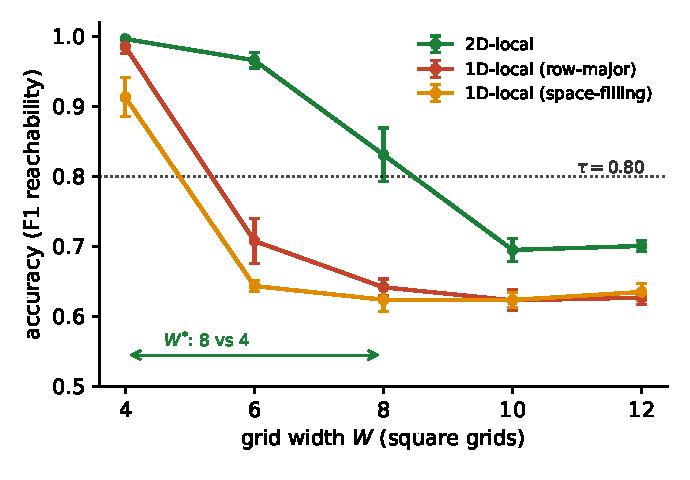
\includegraphics[width=0.62\linewidth]{fig1_bandwidth.pdf}
\caption{\textbf{Bandwidth separation at fixed size} (F1 reachability; 5
seeds, mean $\pm$ s.d.). At matched parameters, window size, and depth, the
2D-local operator clears the $\tau = 0.80$ threshold up to $\Wstar = 8$;
both 1D serializations --- row-major \emph{and} the locality-preserving
space-filling curve --- cap at $\Wstar = 4$, as the grid-bandwidth theorem
predicts.}
\label{fig:bandwidth}
\end{figure}

The outcome, at 5 seeds (Figure~\ref{fig:bandwidth}; per-seed $\Wstar$ in
brackets):

\begin{table}[h]
\centering
\small
\begin{tabular}{lcccccl}
\toprule
$W$ & 4 & 6 & 8 & 10 & 12 & $\Wstar$ (per-seed) \\
\midrule
2D-local & 1.00 & 0.97 & 0.83 & 0.70 & 0.70 & \textbf{8} [8,8,8,8,6] \\
1D-local (row-major) & 0.99 & 0.71 & 0.64 & 0.62 & 0.63 & \textbf{4} [4,4,4,4,4] \\
1D-local (space-filling) & 0.91 & 0.64 & 0.62 & 0.62 & 0.64 & \textbf{4} [4,4,4,4,4] \\
\bottomrule
\end{tabular}
\caption{Fixed-size threshold sweep on F1 (mean accuracy over 5 seeds).}
\label{tab:wstar}
\end{table}

The gap ($+4$) is wide at the crossing ($\Delta \approx 0.19$--$0.26$ at
$W = 6$--$8$), i.e.\ not a threshold artifact, and is seed-stable: both 1D
arms sit at $\Wstar = 4$ in \textbf{every} seed. The per-seed mean-accuracy
advantage over $W \in \{6,8,10,12\}$ is $+0.148 \pm 0.012$ versus row-major
(paired $t = 27.6$, $\pholm = 1.2\times10^{-5}$) and $+0.167 \pm 0.013$
versus the space-filling order ($t = 29.2$, $\pholm = 1.2\times10^{-5}$).

A note on what the theorem does and does not entail. Given a fixed window,
the \emph{direction} of this separation is entailed by the bandwidth bound;
what this section contributes is the measurement under controls. What the
bound does \emph{not} entail: that gradient-trained models
realize the floor cleanly (expressivity does not imply trainability --- our
global baselines are expressive enough for these tasks yet fail to train,
\S\ref{sec:boundary-global}), the magnitude and seed-stability of the gap,
and the transfer phenomena of \S\ref{sec:mech2}--\ref{sec:mech3}, which are
not corollaries of the bound.

\subsection{The serialization objection, defeated empirically}\label{sec:serialization}

The obvious objection --- ``row-major is just a bad order'' --- is what the
space-filling-curve arm answers: the locality-preserving Hilbert-style order,
whose consecutive cells are always grid-adjacent, performs \emph{no better}
than row-major ($\Wstar = 4$, and slightly worse in the working range). This
is the bandwidth theorem made empirical: preserving locality \emph{along} the
curve cannot fix the $\Theta(\min(W,H))$ reach needed \emph{across} it. No
choice of serialization closes the gap.

\subsection{The capacity objection, defeated by the F3 control}\label{sec:capacity}

On the 1D-intrinsic control task the ordering reverses: 1D-local reaches
$\Wstar = 10$ versus 8 for 2D-local (5 seeds; mean 2D$-$1D gap over the sweep
$\mathbf{-0.037}$, two-sided $p = 0.34$ --- no 2D advantage, direction
negative). The 2D arm is not generically stronger; it wins exactly where the
bandwidth analysis says it should, and loses where the task's dependency
structure favors the serialization.

\section{Mechanism II: scale-equivariance and length-generalization}\label{sec:mech2}

The second mechanism is scale-equivariance. A weight-shared 2D-local rule
commutes with changes of grid size: the learned kernel implements the same
one-step interaction on any $W \times H$ field. A 1D serialization breaks
this: the distance between vertically adjacent cells is $W$, so a kernel
calibrated at training width is \emph{semantically miscalibrated} at any
other width. The prediction is that 2D-local rules trained small transfer to
larger unseen sizes, while 1D-local rules do not merely degrade; they
transfer nothing.

To test transfer, we train on mixed $W \in \{4,5,6\}$ and evaluate on unseen
$W \in \{7,\dots,20\}$ (up to $11\times$ the training area). The
pre-registered pass criteria per family: mean 2D$-$1D gap $\ge 0.10$ over
$W \le 10$--$12$, 2D $\ge$ 1D everywhere, and the GNN positive control
$\ge 0.70$ at $W = 8$ (establishing the task \emph{is} length-generalizable
by a scale-free learner).

\begin{figure}[t]
\centering
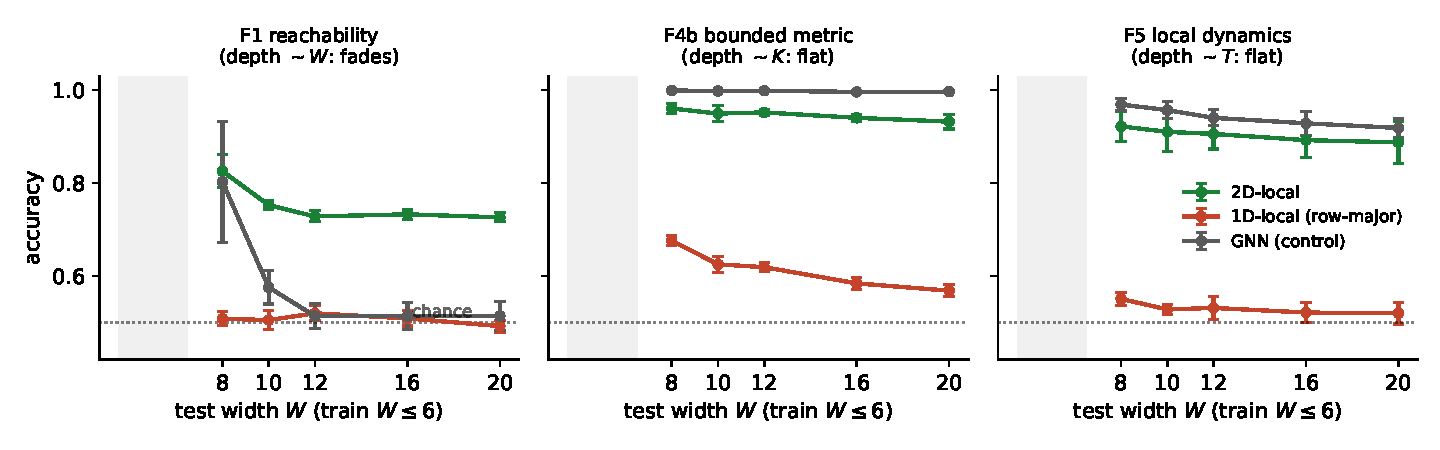
\includegraphics[width=\linewidth]{fig2_lengthgen.pdf}
\caption{\textbf{Length-generalization across the reasoning suite} (train
$W \le 6$, test on unseen $W$; 5 seeds, mean $\pm$ s.d.). The 1D-local arm
transfers nothing (chance-to-weak on every family), while 2D-local transfers
on all three --- flat where intrinsic depth is bounded (F4b, F5) and fading
where required depth scales with $W$ (F1). On F1 the plain fixed-depth GNN
handed the true adjacency satisfies the positive control at $W = 8$ and then
collapses (\S\ref{sec:robustness} evaluates a stabilized recurrent GNN),
while 2D-local holds 0.73 out to $W = 20$.}
\label{fig:lengthgen}
\end{figure}

On reachability (F1), the transfer picture is stark (5 seeds; all test $W$
unseen; Figure~\ref{fig:lengthgen}, left):

\begin{table}[h]
\centering
\small
\begin{tabular}{lccccc}
\toprule
$W$ & 8 & 10 & 12 & 16 & 20 \\
\midrule
2D-local & 0.83 & 0.75 & 0.73 & 0.73 & 0.73 \\
1D-local (row-major) & 0.51 & 0.51 & 0.52 & 0.51 & 0.49 \\
GNN (positive control) & 0.80 & 0.58 & 0.51 & 0.51 & 0.51 \\
\bottomrule
\end{tabular}
\caption{Length-generalization on F1 (mean accuracy over 5 seeds; train
$W \in \{4,5,6\}$).}
\label{tab:f1lengthgen}
\end{table}

The 1D arm is at \emph{chance} on every unseen width --- the strongest single
contrast in this program; the space-filling serialization also fails to
transfer (0.57--0.63 across unseen $W = 7$--$12$ in a 3-seed diagnostic run).
Notably, the plain fixed-depth GNN handed the true adjacency generalizes one
step out (0.80 at $W = 8$, satisfying the positive control) and then
\textbf{collapses} (0.58 at $W = 10$, chance by 12), while 2D-local holds
0.73 out to $W = 20$. We stress what this does and does not show: the
collapse indicts \emph{plain fixed-depth} message passing only, and it is a
stabilization failure rather than anything intrinsic to graph computation ---
adding the standard stabilizers (input skip, GRU state update, $L_2$ state
regularization) repairs it completely (\S\ref{sec:robustness}); a stabilized
recurrent GNN in the style of \citet{groetschla2022recurrent} is evaluated
directly there, and given graphs remain the territory of
\S\ref{sec:boundary-given}.

Across the full suite (train $W \le 6$, test $W = 8 \to 20$, 5 seeds; gap
$=$ per-seed mean of 2D$-$1D over the pre-registered range $W \le 12$), the
same pattern holds in all three families:

\begin{table}[h]
\centering
\small
\begin{tabular}{lcccc}
\toprule
Family (computation type) & 2D-local & 1D-local & gap (mean $\pm$ sd; $\pholm$) & GNN @8 \\
\midrule
F1 reachability (connectivity) & $0.83 \to 0.73$ & $\approx 0.51$ & $+0.258 \pm 0.017$; $9.4\times10^{-6}$ & 0.80 \\
F4b bounded metric ($K = 6$) & $\mathbf{0.96 \to 0.93}$ & 0.57--0.68 & $+0.314 \pm 0.013$; $1.8\times10^{-6}$ & 1.00 \\
F5 local dynamics ($T = 2$) & $\mathbf{0.92 \to 0.89}$ & $\approx 0.53$ & $+0.376 \pm 0.034$; $1.2\times10^{-5}$ & 0.97 \\
\bottomrule
\end{tabular}
\caption{The three-family length-generalization suite (5 seeds).}
\label{tab:suite}
\end{table}

Length-generalization of the 2D-local medium is therefore a \emph{general}
property across connectivity, metric, and dynamics computation, not a quirk
of reachability. A further note on placement: the adversarial source/target
geometry (top row $\to$ bottom row) exists \emph{only} in F1, where it
deliberately exercises the bandwidth mechanism; F4b and F5 place their
queries direction-neutrally at random, and show the \emph{larger} gaps
($+0.314$ and $+0.376$ versus F1's $+0.258$). The advantage does not depend
on rigging the geometry, and \S\ref{sec:robustness} confirms this on F1
itself.

\subsection{What the positive control caught}\label{sec:control-caught}

Our first metric family used a width-coupled threshold ($K = 2(W{-}1)$). The
GNN control \emph{failed} on it (0.56), flagging that the target function
itself was not scale-invariant --- even a scale-free learner cannot transfer a
size-dependent definition. Redesigning with fixed $K$ (F4b) raised the
control to 1.00 and the 2D arm to 0.93--0.96. We report this because it is
easy to mistake such a confound for a model failure; the control isolates
task-side from model-side non-transfer, and we recommend it as standard
practice in length-generalization studies.

\subsection{Robustness: neutral placement and a stronger graph baseline}\label{sec:robustness}

Two checks respond to natural objections to the F1 design (5 and 3 seeds
respectively; raw per-seed data in \texttt{robustness.json}).

\textbf{Placement-neutral F1.} F1's top-row/bottom-row placement deliberately
forces traversal along the high-1D-bandwidth axis; does the advantage require
this rigging? We re-ran the length-generalization protocol on an F1 variant
with source and target placed uniformly at random (same 50/50 balance and
exact wall-count matching). The gap survives decisively: 2D-local
$0.91 \to 0.64$ versus 1D-local $0.59 \to 0.52$ across unseen $W = 8$--$20$;
per-seed mean gap $+0.212 \pm 0.010$ (paired $t = 47.0$,
$p = 6.2\times10^{-7}$, 5 seeds), versus $+0.258$ under the adversarial
placement. The forcing sharpens the contrast; it does not create it.

\textbf{A stabilized recurrent GNN.} Is the \S\ref{sec:mech2} GNN collapse
representative of graph methods? No --- and confirming this with our own data
closes the loop on \S\ref{sec:boundary-given}. We implemented a stabilized
recurrent GNN following \citet{groetschla2022recurrent}: one weight-shared
round with an input skip, an edge MLP, a GRU state update, and $L_2$ state
regularization; variable training rounds and $3W$ rounds at inference;
trained with roughly twice the epoch budget of the other arms, in the same
fair-shot spirit as the Universal Transformer of
\S\ref{sec:boundary-global}. On the original given-graph F1 it
size-generalizes \emph{perfectly} --- \textbf{1.00 at every test width up to
$W = 20$} (3 seeds) --- outperforming every other arm, including 2D-local.
This is the \S\ref{sec:boundary-given} boundary reproduced in-house:
\emph{when the dependency graph is handed to the model, a stabilized
recurrent GNN is the right tool and spatial layout adds nothing}. The
2D-local medium's case is the complementary regime: locality imposed and
structure spatial (positions and fields) rather than given as an edge list.
(The arms also differ in what they must extract: the recurrent GNN receives
wall-aware adjacency, while the local operators must infer connectivity from
the raw field --- so this comparison bounds the value of \emph{being given
the graph}, not architecture alone.)

\section{Mechanism III: a depth taxonomy}\label{sec:mech3}

The suite reveals systematic structure in \emph{how} transfer behaves:

\begin{itemize}
\item \textbf{Bounded intrinsic depth $\Rightarrow$ flat transfer.} F4b needs
  $\sim K$ propagation steps and F5 needs $T$ steps --- independent of $W$.
  Both transfer nearly flat (0.93--0.96 and 0.89--0.92 out to $W = 20$).
\item \textbf{Size-scaling depth $\Rightarrow$ fading transfer.} F1's
  required depth grows like the path length ($\sim W$); under a fixed
  16-layer budget accuracy fades ($0.83 \to 0.73$) as instances outgrow the
  budget.
\end{itemize}

\subsection{Adaptive depth does not (yet) break the bound}\label{sec:adaptive}

The obvious fix --- iterate a weight-shared local update $T \propto W$ times
(a stabilized neural CA with variable-step training) --- was pre-registered
and returned \textbf{null}: the adaptive-depth CA beats the fixed-depth stack
in the mid-range ($+0.11$ to $+0.13$ at $W = 10$--$12$) but ties it at
$W = 16$ (0.72 vs 0.73) and \emph{loses} at $W = 20$ (0.64 vs 0.72),
consistent with drift accumulating over $\sim$60 iterations. Meanwhile the
fixed-depth 2D stack is itself a surprisingly strong flat generalizer
(0.72--0.73 across $W = 8$--$20$). We record this as a real, unbroken
limitation: at this scale, the 2D-local medium's clean transfer story is for
bounded-depth computation; depth-scaling tasks remain budget-limited.

\textbf{Practical reading.} Given a task, ask how its required propagation
depth scales with instance size. Bounded $\Rightarrow$ a small 2D-local model
trained on small instances will transfer essentially flat. Scaling
$\Rightarrow$ expect graceful fading at fixed budget, and do not expect a
naive adaptive-depth CA to fix it.

\section{Boundary conditions: where the advantage does not exist}\label{sec:boundary}

The regime of \S\ref{sec:mech1}--\ref{sec:mech3} is bounded by three negative
results, each pre-registered.

\subsection{Remove locality and the advantage vanishes}\label{sec:boundary-global}

In an earlier pilot study we tested 2D structure as an \emph{input
encoding} under global attention: absolute Fourier positional features,
relative-position attention biases, and a translation-invariant
mean-centering model, on node-link relational tasks. All three converged on
\textbf{2D-versus-set $\approx 0$} (e.g.\ $-0.013$ / $+0.012$ / $-0.058$
across task families under translation shift): set attention is already
robust where 2D structure was supposed to help, and the only large effect was
the known set $\gg$ sequence gap. Within the present program we made three attempts at a capable
iterative-global baseline on F1. A $16\times$-looped transformer failed to
train at all (chance at every width), and a parameter-matched stabilized
Universal Transformer reached only 0.70 even at trivial $W = 4$. The third
attempt succeeded: with a width curriculum ($W = 4 \to \{4,5\} \to
\{4,5,6\}$), learning-rate warmup, and hidden width 64, the same Universal
Transformer trains to 0.84 mean accuracy on $W \in \{4,5,6\}$ (3 seeds), and
then transfers \emph{nothing}: 0.68 at $W = 8$, 0.55 at $W = 12$, and
chance (0.52--0.53) at $W \in \{16, 20\}$, while the 2D-local arm trained on
the same widths holds 0.73 at $W = 20$
(Table~\ref{tab:f1lengthgen}). The boundary therefore no longer rests on a
training failure: at this scale, a \emph{trained} iterative-global model
matches the local arms in distribution --- where, per the input-encoding
pilot above, layout is irrelevant --- and cedes the entire length-generalization axis to
the 2D-local medium. Global attention erases the layout advantage \emph{at
the sizes it is trained on}; it does not inherit the scale-transfer that
locality provides. (Caveats: one recipe at hidden width 64; the iteration
count is architecturally fixed at 16 by the per-step embeddings, so unlike
the recurrent arms this model cannot run longer at test time; larger-scale
global models remain untested, \S\ref{sec:limitations}.)

\subsection{Given the graph, layout is unnecessary}\label{sec:boundary-given}

\citet{groetschla2022recurrent} show recurrent GNNs with skip connections,
state regularization, and edge convolutions extrapolate path, prefix-sum, and
distance tasks to graphs $1000\times$ training size. We treat this as a
boundary rather than a competitor: \textbf{when the sparse dependency graph is
handed to the model, size-generalizing iterative computation is achievable
with no spatial layout at all.} Our \S\ref{sec:robustness} arm reproduces
this in-house: a stabilized recurrent GNN reaches 1.00 at every test width on
given-graph F1. A 2D re-embedding can only add value when the graph is
\emph{not} given --- which motivated the final experiment.

\subsection{Learning the layout loses to a set-transformer}\label{sec:boundary-layout}

We built the implicit-structure case: a latent $W \times W$ grid with a
smooth land/water field; input is an \emph{unordered set} of cells with
affinely scrambled coordinates (rotation $+$ shear $+$ noise; recoverable but
not given), no adjacency list; the label is whether two marked cells share a
4-connected land component. The layout arm encodes the set, predicts per-cell
positions, soft-assigns cells to lattice sites via Sinkhorn
\citep{cuturi2013sinkhorn, mena2018gumbel}, and runs the \S\ref{sec:mech2}
local-CA --- trained end-to-end (gradients flow through the placement;
verified). Controls: a set-transformer, a kNN-graph recurrent GNN, and a
\emph{random-layout} arm (same lattice $+$ CA, placement not learned).

Result (train $W \in \{6,8\}$, test $W \in \{12,16,20\}$; re-run at
\textbf{5 seeds} with a $1.5\times$ epoch budget for this paper --- the
original pre-registered gate used 3 seeds and reached the same verdict): the
learned layout extracts real structure --- it beats random layout by $+0.11$
at $W = 20$ and transfers flat ($0.65 \to 0.62$) --- but it \emph{underfits}
(0.65 at train size vs 0.70--0.71 for the baselines), and the set-transformer
is flat \textbf{and higher} (0.70 everywhere; $-0.08$ ahead at $W = 20$).
Notably, the extra budget helped the baselines (set-transformer $0.67 \to
0.70$ versus the 3-seed run) but not the layout arm --- the underfit is
specific to the joint placement$+$execution objective, not a global
training-budget artifact. Two of three pre-registered criteria fail
$\Rightarrow$ null. One secondary observation survives: the kNN-graph arm
\emph{degrades} at scale ($0.71$--$0.73 \to 0.63$--$0.65$) while lattice and
attention stay flat --- regular structure transfers, data-dependent graphs
degrade.

\textbf{Boundary statement.} The joint ``infer the layout, then exploit it
locally'' problem is where the 2D-medium program currently stops: the
placement is trainable but not yet competitive with a strong set baseline.
This is the third independent reproduction (after the notation-utility and
input-encoding pilots) of the pattern that permutation-invariant attention is
the baseline to beat, and it usually is not beaten.

\section{A decision procedure}\label{sec:decision}

For a practitioner asking ``should I use a 2D-local medium for this task?''
(Figure~\ref{fig:decision}). Two notes on evidential status: the procedure
synthesizes our controlled results, and its steps rest on evidence of
differing strength --- step 1 on a trained-global comparison at pilot scale
(\S\ref{sec:boundary-global}) and step 3 on a 5-seed null
(\S\ref{sec:boundary-layout}); and two of its branch recommendations have
been checked out-of-sample on external benchmarks (\S\ref{sec:external}).

\begin{enumerate}
\item \textbf{Is your compute constrained to local operators} (hardware,
  latency, $O(N)$-per-step budgets, or an architectural choice like
  CA/conv)? If no --- if global attention is affordable and trainable on your
  task --- the layout will not matter in-distribution
  (\S\ref{sec:boundary-global}). If train-small$\to$run-large transfer is
  itself the requirement, however, note that even our \emph{trained} global
  ceded that axis (\S\ref{sec:boundary-global}); locality then re-enters as
  the route to transfer.
\item \textbf{Is the dependency structure given explicitly} (edge lists)? If
  yes, use a recurrent GNN with stabilization; layout adds nothing
  (\S\ref{sec:boundary-given}).
\item \textbf{Is the structure natively 2D or reliably embeddable} (grids,
  images, boards, physical fields, spatial programs)? If it must be
  \emph{learned} from implicit structure, expect a set-transformer to win at
  current recipes (\S\ref{sec:boundary-layout}).
\item \textbf{Is the dependency bandwidth low in 2D but high in 1D}
  (interactions spatially adjacent, no serialization keeps them adjacent)?
  If the task is 1D-intrinsic, serialize it (\S\ref{sec:capacity}).
\item \textbf{Does required depth scale with instance size?} Bounded
  $\Rightarrow$ expect flat length-generalization from a small trained model
  (\S\ref{sec:mech3}). Scaling $\Rightarrow$ expect fading at fixed depth;
  adaptive-depth CAs do not currently fix this (\S\ref{sec:adaptive}).
\end{enumerate}

Yes to 1, 3, 4 (and ideally ``bounded'' at 5) is the regime where the
2D-local medium is, in our data, decisively the right prior --- with per-step
cost $O(N \cdot k)$ versus $O(N^2)$ for attention, and training possible
entirely on small instances. Natural application domains are native-grid
computation under locality constraints: spatial accelerators and
systolic-style hardware mappings, cellular/field simulations, and grid-based
reasoning benchmarks.

\begin{figure}[t]
\centering
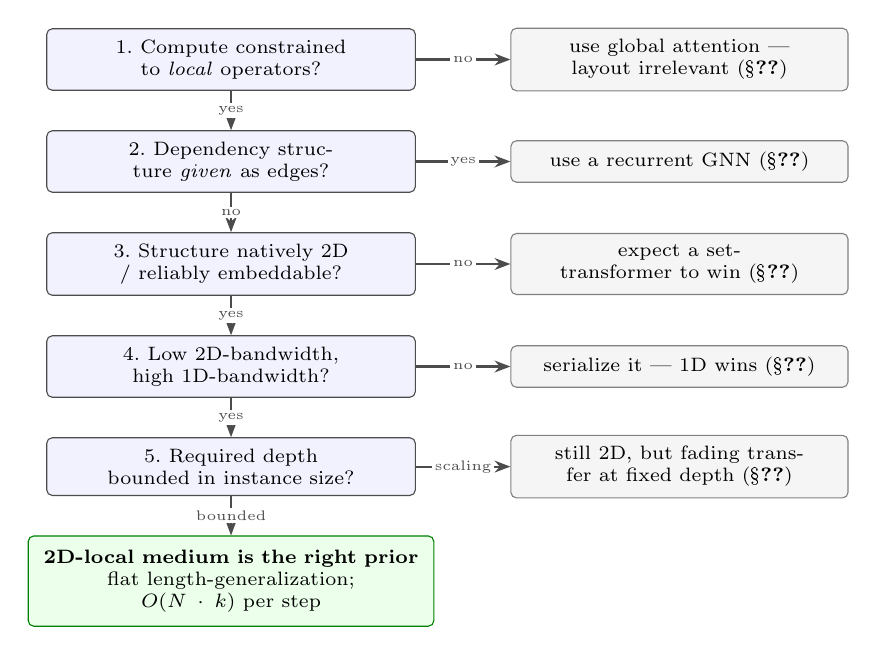
\begin{tikzpicture}[
  font=\scriptsize,
  q/.style={rectangle, rounded corners=2pt, draw=black!70, fill=blue!5,
            text width=44mm, align=center, inner sep=4pt},
  outcome/.style={rectangle, rounded corners=2pt, draw=black!50, fill=black!4,
              text width=40mm, align=center, inner sep=4pt},
  win/.style={rectangle, rounded corners=2pt, draw=green!50!black,
              fill=green!8, text width=48mm, align=center, inner sep=5pt},
  lab/.style={font=\tiny, fill=white, inner sep=1pt},
  arr/.style={-{Stealth[length=2mm]}, thick, black!70},
  node distance=5mm and 12mm]

\node[q] (q1) {1.\ Compute constrained to \emph{local} operators?};
\node[q, below=of q1] (q2) {2.\ Dependency structure \emph{given} as edges?};
\node[q, below=of q2] (q3) {3.\ Structure natively 2D / reliably embeddable?};
\node[q, below=of q3] (q4) {4.\ Low 2D-bandwidth, high 1D-bandwidth?};
\node[q, below=of q4] (q5) {5.\ Required depth bounded in instance size?};
\node[win, below=of q5] (win) {\textbf{2D-local medium is the right prior}\\
  flat length-generalization; $O(N \cdot k)$ per step};

\node[outcome, right=of q1] (o1) {use global attention --- layout irrelevant
  (\S\ref{sec:boundary-global})};
\node[outcome, right=of q2] (o2) {use a recurrent GNN
  (\S\ref{sec:boundary-given})};
\node[outcome, right=of q3] (o3) {expect a set-transformer to win
  (\S\ref{sec:boundary-layout})};
\node[outcome, right=of q4] (o4) {serialize it --- 1D wins
  (\S\ref{sec:capacity})};
\node[outcome, right=of q5] (o5) {still 2D, but fading transfer at fixed depth
  (\S\ref{sec:adaptive})};

\draw[arr] (q1) -- node[lab] {yes} (q2);
\draw[arr] (q2) -- node[lab] {no} (q3);
\draw[arr] (q3) -- node[lab] {yes} (q4);
\draw[arr] (q4) -- node[lab] {yes} (q5);
\draw[arr] (q5) -- node[lab] {bounded} (win);
\draw[arr] (q1) -- node[lab] {no} (o1);
\draw[arr] (q2) -- node[lab] {yes} (o2);
\draw[arr] (q3) -- node[lab] {no} (o3);
\draw[arr] (q4) -- node[lab] {no} (o4);
\draw[arr] (q5) -- node[lab] {scaling} (o5);
\end{tikzpicture}
\caption{\textbf{The decision procedure} distilled from the mechanism and
boundary results: five questions predicting whether a 2D-local computational
medium will help on a given task.}
\label{fig:decision}
\end{figure}

\subsection{Out-of-sample checks of the procedure}\label{sec:external}

The procedure synthesizes our own controlled experiments; a fair objection is
that it had never been tested on data we did not design. We checked two of
its branch recommendations on external benchmarks.

\textbf{Given-graph branch (step 2) --- official CLRS-30 BFS.} Using the
benchmark's own sampler (\texttt{dm-clrs} 2.0.3;
\citealp{velickovic2022clrs}), we trained at the standard size $n = 16$ and
evaluated pointer accuracy at $n \in \{16, 32, 64\}$ (3 seeds). The step-2
recommendation --- use a stabilized recurrent GNN; no layout --- holds
exactly: the \S\ref{sec:robustness}-style RecGNN reaches
$1.00 / 1.00 / 0.95$, while a plain fixed-depth MPNN degrades
($0.98 / 0.91 / 0.58$) --- reproducing the in-house plain-versus-stabilized
contrast on official benchmark data.

\textbf{Native-2D branch (steps 3--5) --- Schwarzschild et al.\ mazes.} On
the easy-to-hard maze benchmark \citep{schwarzschild2021canyou} (predict the
optimal-path mask; the metric is full-maze accuracy), our pilot-scale budget
is far below the benchmark's demands: at this paper's standard budget both
local arms score zero full-maze accuracy. Under a fair-shot scale-up (depth
48, hidden 64, 50 epochs, 20k mazes; 1 seed, exploratory), the predicted
ordering emerges on the benchmark's own metric: the 2D-local arm solves
11\% of held-out $9 \times 9$ mazes with 0.97 pixel accuracy and fades to
zero by $13 \times 13$, while the matched 1D arm solves \emph{none at any
size}, its pixel accuracy stuck at the all-background floor (0.85--0.87).
This is the procedure's own step-5 warning made concrete: the task's
required depth scales with maze size, so a fixed-depth model cannot master
it --- mastery on this benchmark is achieved by test-time-extendable
recurrence \citep{schwarzschild2021canyou}, consistent with our depth
taxonomy (\S\ref{sec:mech3}). The external check therefore confirms the
\emph{ordering} claim (2D-local $\gg$ matched 1D at every size, on a task we
did not design) and the step-5 depth caveat; absolute benchmark mastery at
pilot scale was not achieved, and we report it as such.

\section{Limitations}\label{sec:limitations}

\begin{itemize}
\item \textbf{Pilot scale.} Hidden width 32 and synthetic binary tasks
  throughout. The statistical base is hardened but small: all load-bearing
  comparisons were re-run at 5 seeds with per-seed records; the five headline
  effects are significant under Holm correction (all
  $\pholm < 2\times10^{-5}$, one-sided paired $t$, $t \in [24.7, 53.5]$);
  per-seed $\Wstar$ distributions are reported in \S\ref{sec:mech1} (both 1D
  arms at $\Wstar = 4$ in every seed); and every pre-registered gate
  re-checked unchanged on the 5-seed means (none flipped). Larger models and
  wider task batteries remain untested.
\item \textbf{Task breadth.} The mechanism families are synthetic and
  designed to isolate bandwidth. Two out-of-sample checks on external
  benchmarks (\S\ref{sec:external}: official CLRS-30 BFS; the Schwarzschild
  maze benchmark) now bound this concern but do not remove it; broader
  batteries remain future work, and the maze check in particular is 1-seed
  exploratory with pilot-scale absolute performance.
\item \textbf{The capable-global comparison is partially closed.} After two
  training failures, a curriculum-trained Universal Transformer learns F1
  in-distribution and fails to length-generalize
  (\S\ref{sec:boundary-global}), so the boundary now rests on a trained
  model at pilot scale. What remains untested is scale: whether much larger
  global models --- cf.\ the scale-trumps-inductive-bias lesson of
  \citet{dosovitskiy2021vit} --- would close the transfer gap.
\item \textbf{Supervised, hand-designed substrate.} All results concern what
  structure a learner can \emph{exploit}, not what it can \emph{discover};
  the learned-layout null (\S\ref{sec:boundary-layout}) marks the current
  frontier of the latter, and our separate multi-year program on emergent 2D
  communication closed negative (14 pre-registered nulls), which we treat as
  out of scope here.
\item \textbf{Two dimensions specifically.} We did not test 3D or higher; the
  bandwidth argument generalizes (bandwidth of a $d$-dimensional lattice
  under $(d{-}1)$-dimensional layouts) and is an obvious extension.
\end{itemize}

\section{Conclusion}\label{sec:conclusion}

Whether a 2D layout helps a neural network reason is not one question but
three, and they have different answers. As an input encoding under global
attention: no. As a representation to be learned from implicit structure: not
yet --- a set-transformer remains the wall. As a \emph{computational medium}
under a locality constraint: yes, decisively, and for stateable reasons: a
bandwidth separation that no serialization can close, a scale-equivariance
that turns small-instance training into large-instance competence, and a
depth taxonomy that predicts when that competence is flat. In slogan form,
locality gates dimensionality: 2D layout is a precise reasoning prior rather
than a general one, and we provide the map of where it pays.

\subsection*{Reproducibility}

All stages were pre-registered in-repo before execution, with raw per-seed
results as JSON alongside; the statistical-hardening data
(\texttt{harden\_stats.json}) accompanies the code. Experiments run on a
single laptop-class accelerator; every original pre-registered stage took
under $\sim$25 minutes, while the heaviest revision re-run (the 5-seed
hardening of the learned-layout gate, executed under contention) took
$\sim$11 hours. Code, pre-registrations, and raw per-seed results are
available at
\url{https://github.com/sakatani/locality-gates-dimensionality}.

\bibliographystyle{plainnat}
\bibliography{refs}

\end{document}
